\documentclass[12pt,titlepage]{report}
%\usepackage[authoryear,semicolon]{natbib}
\usepackage{pdfpages}
%\usepackage{chicago}
\usepackage[onehalfspacing]{setspace}
%\doublespacing
%\linespread{1.6}
\setstretch{1.5}
\usepackage{apalike}
\onehalfspacing
\usepackage[left=40mm,right=25mm,top=30mm,bottom=20mm,headsep=10mm]{geometry}
\geometry{a4paper}
\usepackage[titletoc]{appendix}
\usepackage{fnpara}
\usepackage{graphicx}
\usepackage{epstopdf}
%\usepackage{mathtools}
\usepackage{amsmath,amsfonts,amsthm,amssymb}
\usepackage{fancybox}

%\usepackage[active]{srcltx}
\usepackage{afterpage}
\usepackage[mathscr]{eucal}
\DeclareGraphicsRule{.tif}{png}{.png}{`convert #1 `dirname
#1`/`basename #1 .tif`.png}
%\usepackage{fancyhdr}
%\pagestyle{fancy}
%\fancyhf{}
%\rhead{ \leftmark}
%\rhead[\thepage]{\chaptermark}
%\lhead{Oyebamiji, O.K.}
%\cfoot{ \thepage}


\usepackage{setspace}
\usepackage[small]{caption}
\usepackage{color}
\usepackage{subcaption}
\usepackage{placeins}
\usepackage{epstopdf}
\usepackage{booktabs}
\usepackage{tikz}
\usepackage{subcaption}
%\usepackage{color,framed} %Utilisation des couleurs et de l'environnement shaded
%\definecolor{shadecolor2}{rgb}{.92,.92,.92} % choix de la teinte de ``shaded''
%\definecolor{shadecolor}{rgb}{.6,.95,.6} % choix de la teinte de ``shaded''
\usepackage[pagebackref=true,colorlinks=true, linkcolor=black,anchorcolor=blue,citecolor=black,filecolor=blue,menucolor=blue,
urlcolor=black,plainpages=false,pdfpagemode=UseThumbs,pdftitle={Titre},pdfauthor={oluwole},
pdfsubject={Thesis},pdfstartview=FitH]{hyperref} % Extensions PDF



%=========Standard sets===========:
\newcommand{\stsets}[1]{\mathbb{#1}}
\newcommand{\R}{\stsets{R}}
\newcommand{\N}{\stsets{N}}
\newcommand{\C}{\stsets{C}}

%===============Theorems etc.========================
%Paul
\newcommand{\bt}{{\bf t}}
\newcommand{\bB}{{\bf B}}
\newcommand{\bSigma}{{\bf \Sigma}}
\newcommand{\tbSigma}{{\tilde {\bf \Sigma}}}
\newcommand{\tbu}{{\tilde {\bf u}}}
\newcommand{\tbU}{{\tilde {\bf U}}}
\newcommand{\bh}{{\bf h}}
\newcommand{\bH}{{\bf H}}
\newcommand{\bD}{{\bf D}}
\newcommand{\bU}{{\bf U}}
\newcommand{\bu}{{\bf u}}
\newcommand{\bZ}{{\bf Z}}
\newcommand{\bz}{{\bf z}}
\newcommand{\bC}{{\bf C}}
\newcommand{\bc}{{\bf c}}
%%
\newcommand{\bx}{{\bf x}}
\newcommand{\bX}{{\bf X}}
\newcommand{\by}{{\bf y}}
\newcommand{\bY}{{\bf Y}}
\newcommand{\bE}{{\bf E}}
\newcommand{\bW}{{\bf W}}
\newcommand{\tbx}{{\tilde {\bf x}}}
\newcommand{\tbX}{{\tilde {\bf X}}}
\newcommand{\tby}{{\tilde {\bf y}}}
\newcommand{\tbY}{{\tilde {\bf Y}}}
\newcommand{\hbX}{{\hat {\bf X}}}
\newcommand{\hbY}{{\hat {\bf Y}}}
\newcommand{\hby}{{\hat {\bf y}}}
\newcommand{\ty}{{\tilde {y}}}
\newcommand{\hy}{{\hat {y}}}
\newcommand{\bs}{{\bf s}}


\newcommand{\bLambda}{\mathbf{\Lambda}}
\newcommand{\bGamma}{\mathbf{\Gamma}}
\newcommand{\hbGamma}{\hat {\mathbf{\Gamma}}}

\newcommand{\bgamma}{{\boldsymbol{\gamma}}}
\newcommand{\bepsilon}{{\boldsymbol{\varepsilon}}}
\newcommand{\tbepsilon}{{\tilde{\boldsymbol{\varepsilon}}}}
\newcommand{\hbepsilon}{{\hat{\boldsymbol{\varepsilon}}}}
\newcommand{\bbeta}{{\boldsymbol{\beta}}}
\newcommand{\hbbeta}{{\hat{\boldsymbol{\beta}}}}
\newcommand{\btau}{{{\boldsymbol{\tau}}}}

\theoremstyle{definition}
\newtheorem{definition}{Definition}
\theoremstyle{remark}
\newtheorem{remark}[definition]{Remark}
\newtheorem{example}[definition]{Example}

%\newtheoremstyle{mytheorem}{0.5cm}{0.2cm}{\slshape}{ }{\bfseries}{.}{}{}
%\theoremstyle{my theorem}
\newtheorem{Th}[definition]{Theorem}
%\newtheorem{Prop}[definition]{Proposition}
\newtheorem{lemma}[definition]{Lemma}
\newtheorem{Cor}[definition]{Corollary}
%\restylefloat{figure}

%==========Probabilistic===========:
%\renewcommand{\cite}{\shortciteN}
\renewcommand{\P}{\mathbf{P}}
\renewcommand{\Re}{\mathrm{Re\,}}
\renewcommand{\Im}{\mathrm{Im\,}}
%\newcommand{\Prob}[1]{\mathbf{P}\{#1\}}
\DeclareMathOperator{\E}{{\bf E}}
\DeclareMathOperator{\var}{{\bfvar}}
\DeclareMathOperator{\supp}{supp}
\DeclareMathOperator{\dist}{dist}
\DeclareMathOperator{\one}{{1\hspace*{-0.55ex}I}}
%\DeclareMathOperator{\one}{{\mathbf{1}}}
\newcommand{\Ind}[1]{\one_{#1}}
\newcommand{\cond}{\hspace*{1ex} \rule[-1ex]{0.15ex}{3ex}\hspace*{1ex}}

%==========Divers===========:
\DeclareMathOperator*{\ssum}{{\textstyle \sum}}
%small\sum for\sum\delta_x
\newcommand{\comp}{\mathbf{c}}
\newcommand{\mydot}{{\raisebox{.3ex}{$\scriptscriptstyle{\,\bullet\,}$}}}
%\newcommand{\myline}{\newline\underline{\hskip\textwidth}}
\newcommand{\mytimes}{\!\times\!}
\newcommand{\mytilde}{{\!\raisebox{-0.9ex}{$\tilde{\ }$}}}
\renewcommand{\epsilon}{\varepsilon}
\renewcommand{\vec}[1]{\mathbf{#1}}
%\renewcommand{\phi}{\varphi}
\newcommand{\ti}{\to\infty}
\newcommand{\ssp}{\hspace{2pt}}
\newcommand{\seg}{see, \hbox{e.\ssp g.,}\ }
\newcommand{\ie}{\hbox{i.\ssp e.}\ }
\newcommand{\eg}{\hbox{e.\ssp g.,}\ }
\newcommand{\cf}{\hbox{c.\ssp f.}\ }
\newcommand{\etc}{\hbox{etc.}\ }
\newcommand{\iid}{\hbox{i.\ssp i.\ssp d.}\ }
\newcommand{\as}{\hbox{a.\ssp s.s}\ }
\newcommand{\viz}{\hbox{viz.}\ }
\renewcommand{\bibname}{References}
\renewcommand{\abstractname}{Abstract}


%\pagenumbering{roman}

\begin{document}
\chapter*{Emulation of Lammp outputs}
We describe the procedure for building a simple emulator of Lammp output.
%\section*{Lammp emulator}
\subsection*{Experimental design}
This section describes the procedure for generating the parameter combinations and variables at which the Lammp model is run. We run the Lammp code for a small sample of inputs using a Latin Hypercube Design (LHD). This produces data for training the Lammp emulator to approximate the major Lammp outputs. LHD provides a good coverage of the input space with relatively small number of design points. We use maximin LHS technique that optimises samples by maximizing the minimum distance between design points. Suppose we want to sample a function of $p$ variables, the range of each variable is divided into $n$ probable intervals, $n$ sample points are then drawn such that a Latin Hypercube is created.

We generate an $n \times p$ variables Latin Hypercube sample matrix with values uniformly distributed on interval [0,1]. We then transformed the generated sample matrix to the quantile of a uniform distribution using the range of the parameters given in Table \ref{mytab1}. We limit our initial analysis to just $n=100$ training points for each dimension of the $p=22$ input spaces that are to be varied because Lammp model are computationally demanding. %The inversion of the correlation matrix under GP regression becomes more difficult as we increase the number of training points. 

%(in this report, we consider only mean floc diameter)

\subsection*{Simulation data}
We describe 2 different simulation procedures. Firstly, let the design matrix which contain the input to the Lammp model be denoted by $D=(\theta^i_p, t_p, p=1,\ldots,22; i=1,\ldots,100)$, where the subscript $p$ represents the 22 input parameters and superscript $i$ denote 100 different realisations (design points), $t_p$ is the time in seconds at which the output data is recorded. The design matrix $D_{100 \times 23}$ denotes the input values at which the Lammp model will be run for every combinations of $x_p$ where $x_p$ represents $p^{th}$ row of $D$. The current Lammp code is set up to produce the following outputs namely particle diameter, position (3-dimensional), velocity (3-dimensional) and force (3-dimensional). The Lammp code could be run for as long as there are sufficient computing resources to store the outputs. For the present analysis, the code is run for 352800 seconds to generate sufficient data for the emulation which is equivalent to $\approx$ 4 days of real time and generated output results are saved at a time-step of 2000 seconds which gives about 176 different time slices. 

Therefore, a single run of the code for each of design point $x_p$ will produce 10 different outputs and 176 time steps. There are 5 different types of particle in the simulation namely AOB, NOB, HET, EPS and inert. We note that the shape and number of particles as well as the composition of the floc at each time step vary in the simulation. 

We perform the second simulation using the same input configuration as described above but repeated the runs for 5 times in order to incorporate stochastic variations in our outputs. This of course increases the amount of CPU time for the entire simulations even with running the bash script in parallel on a Linux machine. 


%\section*{Methods}
\subsection*{Procedure}
The work focuses on predictions of mean floc diameter from Lammp simulation outputs together with their associated uncertainty levels. We proposed a two-stage approach where we combined a linear model in the first stage and a Gaussian process regression for residual interpolation in the second stage.

Here, we describe the procedure for emulating the particle floc diameter. We start by computing the average diameter of all the particles at each time step to obtain a vector $\by(x)=\bar z_1,\ldots,\bar z_{176}$ of the mean floc diameter to be emulated such that
\begin{equation}
\bar z_t=\frac{\sum^N_{k=1} z_{kt}}{N}
\end{equation}
where $k=1,\ldots, N$, $N$ represents the total number of all 5 particles at each time slice and varies across time point and $z_{kt}$ is a simulation particle $k$ at time $t$.
For the training data, we sub-sample 75 out of 176 time slices for each design point $x_p$ which gives a total of 7500 observations.
The training data are ($7500 \times 1$) vector of mean floc diameter $\by$ of Lammp output and ($7500 \times 23$) matrix $\bX$, which holds the values taken by the explanatory variables. (NOTE: sequence of time $t$ at which output is sought is used as an additional input to the emulator). We fit a linear model to data $[\by,\bX]$ and then obtain the predictions $\hby$.
We also use the fitted model to predict the left out observations $\tby^{new}$ for cross validation purpose and standard error of predictions $\bs^{new}$ of which is a measure of prediction uncertainty in the linear model. Finally, we apply a GP to model the residual field obtaining from the linear model.
To construct our emulator for the prediction of floc diameter, we fit a linear model to the data in the first stage using equation (\ref{geneq}) and apply a Gaussian process regression for residual analysis
\begin{equation}\label{geneq}
\by=f(\textbf{X})+\boldsymbol\varepsilon= \beta'_0+\beta'_{1}\bx_{1}+\ldots +\beta'_{p}\bx_{p}+\boldsymbol\varepsilon
\end{equation}
where $\by$ is the Lammp simulated mean floc diameter, $p=23$ is the number of parameters for estimation and $\bx_1,\ldots,\bx_p$ are independent variables and $\beta'_1,\ldots,\beta'_{23}$ are regression coefficients. We assume $\boldsymbol \varepsilon \sim N(0, \sigma^2)$. 

\subsection*{Stage 2: GP modelling of residual data}
The (${7500\times 1}$) vector of training residual $\boldsymbol \varepsilon=\by-\hby$ can be modelled as $\boldsymbol \varepsilon= \eta(X')$. We use standardized regression coefficients of equation (\ref{geneq}) as a measure of sensitivity to select important explanatory variables for the GP regression such that $X'<< X$ ($p$ is now $<23$).
Since Gaussian process is described completely by its mean and covariance functions, the mean function is given as
\begin{equation}\label{eqgp3}
E[\eta(X')|\boldsymbol\beta]=h^{\rm T}(\bX')\boldsymbol\beta,
\end{equation}
where $h(\bX')$ is a vector of regression functions. For our analysis, we use a simple linear function $h(\bX') = (1,\bx^T$) and $\boldsymbol\beta$ is an unknown hyperparameter to be estimated and covariance function $$ K={Cov[\eta(\bx),\eta(\bx')|\sigma^{2},\boldsymbol \alpha]=\sigma^{2} \bC(\bx,\bx^{\rm T})},$$ where $\sigma^{2}$ is a noise variance and $\bC(\bx,\bx^{\rm T})$ is a correlation function with an hyperparameter $\boldsymbol \alpha$. We use a Gaussian correlation function of the form
\begin{equation}
\bC=\Big \{\exp(-(x-x')^T \boldsymbol \alpha (x-x')) \Big\}%\exp^{\Big[\sum \limits_{j=1}^{4}{-\boldsymbol \alpha_j(\bx_{j}-\bx^{\rm T}_{j})^2}\Big]}.
\end{equation}
It is difficult to apply a GP directly to the entire residual data because of the inversion of covariance matrix which scales cubically with the number of
observations O($N^3$), we proceed by randomly sub-sampling just 200 observations from the data and denote the training data as $[\by, \bX']$, where $\by=[ \varepsilon_1= \eta(x_1),\ldots, \varepsilon_{200}= \eta(x_{200})]$. We select just 4 explanatory variables for the GP modelling and our correlation parameter is denoted as $\boldsymbol \alpha=(\alpha_1,\ldots,\alpha_4)$.

We assign a non-informative prior to the $\boldsymbol \beta$ and $\sigma^2$ parameters and update these prior distributions with respect to some data $\by$, in order to obtain the posterior estimates using Bayes theorem. We estimate their values by conditioning on each parameter and maximize the resulting marginal likelihood function. Therefore, the posterior distribution of $\eta(.)|\by \sim N\Big \{\mu^{\star}, K^{\star} \Big\}$, where

\begin{equation}\label{olu1}%\tag{A.8}\label{olu1}
\mu^{\star}(\mathbf{x})=h(\mathbf{x})^T\boldsymbol{\hat\beta}+t(\mathbf{x})^T\bC^{-1}[\by-\bH\boldsymbol{\hat\beta}]
\end{equation}
\begin{multline}\label{olu2}%\tag{A.9}\label{olu2}
\begin{split}
K^{\star}=\hat \sigma^2 \Big \{c(\mathbf{x,x'}) -t(\mathbf{x})^T\bC^{-1} t(\mathbf{x}) + \\ \Big ( h(\mathbf{x})^T-t(\mathbf{x})^T\bC^{-1}t(\mathbf{x}) \Big )
(\bH^T\bC^{-1}\bH)^{-1}\Big ( h(\mathbf{x'})^T-t(\mathbf{x'})^T\bC^{-1}t(\mathbf{x'}) \Big )^T
\Big \}
\end{split}
\end{multline}
where $t(\mathbf{x})^T=[c(\mathbf{x},\mathbf{x_1}),\ldots, c(\mathbf{x},\mathbf{x_n})]$ and $\bH^T=[h(\mathbf{x}_1),\ldots, h(\mathbf{x}_n)]$ see more details in the appendix. We analyse our results using "emulator" package in $R$.

Finally, let the GP posterior mean and variance estimates of the residual at a new input point (crossvalidation) be denoted as $\mu^{\star \star}$ and $K^{\star \star}$ respectively, and predictions and standard error of predictions from linear model as $\tby^{new}$ and $\bs^{new}$ respectively. The final predictions of mean particle diameter $\hby^{new}$ is given as
\begin{equation}\label{r1}
\hby^{new} = \tby^{new} +\mu^{\star \star}(\bx)
\end{equation}
and total uncertainty is
\begin{equation}\label{r1}
\hat \bs^{new} = \bs +\sqrt{|K^{\star \star}}|
\end{equation}

\begin{table}
\caption{List of all the parameters}\label{mytab1}
\centering
\fbox{
\begin{tabular}{*{2}{c|c|c}}
Index&Parameters& Value\\ 
\hline
1&variable KsHET &0.01\\
2&variable Ko2HET & 0.81\\
3&variable Kno2HET & 0.0003\\
4&variable Kno3HET & 0.0003\\

5&variable Knh4AOB & 0.001\\
6&variable Ko2AOB & 0.0005\\

7&variable Kno2NOB & 0.0013\\
8&variable Ko2NOB & 0.00068\\


%#Defining maximum growth variables: list from Jaya 
9&variable MumHET & 0.00006944444\\
10&variable MumAOB & 0.00003472222\\
11&variable MumNOB & 0.00003472222\\
12&variable etaHET & 0.6\\

%#Defining decay rates variables: list from Jaya 
13&variable bHET & 0.00000462962\\
%#variable bHET & 0.00462962\\
14&variable bAOB & 0.00000127314\\
%#variable bAOB & 0.00127314\\
15&variable bNOB & 0.00000127314\\
%#variable bNOB & 0.00127314\\
16&variable bEPS & 0.00000196759\\

17&variable YEPS & 0.18\\
18&variable YHET & 0.61\\
19&variable EPSdens & 30\\
20&variable EPSratio & 1.25\\

21&variable factor & 1.5\\
22&variable ke & 5e+10
\end{tabular}}
\end{table}


These are summary of steps taken for emulating Lammp output:
\begin{itemize}
\item[{(i)}] Design of experiment to identify important outputs (which outputs are to be emulated). 
\item[{(ii)}] Determine the relevant input factors to be varied (use all the 22 factors for now). 
\item[{(iii)}] Assign uniform probability density to each input variable (we have little knowledge about these parameters). 
\item[{(iv)}] Generate LHS of 100 design points on each of the 22 input parameters and transform into the quantile of uniform distribution using parameter ranges in Table \ref{mytab1}. 
\item[{(v)}] Evaluate Lammp model for various input combinations to obtain the training data.
\item[{(vi)}] Compute the Lammp mean floc diameter for each time-step
\item[{(vii)}] Randomly sample 75 time points out of 176 for each design point
\item[{(viii)}] Fit a linear model with equation (\ref{geneq}) using all 23 parameters (time included as additional variable to the linear model)
\item[{(ix)}] Obtain both predictions and standard error of predictions for all scenarios
\item[{(x)}] Perform the GP emulation on the unexplained residual data
\end{itemize}

\begin{figure}
        \centering
        \begin{subfigure}[h]{\textwidth}
           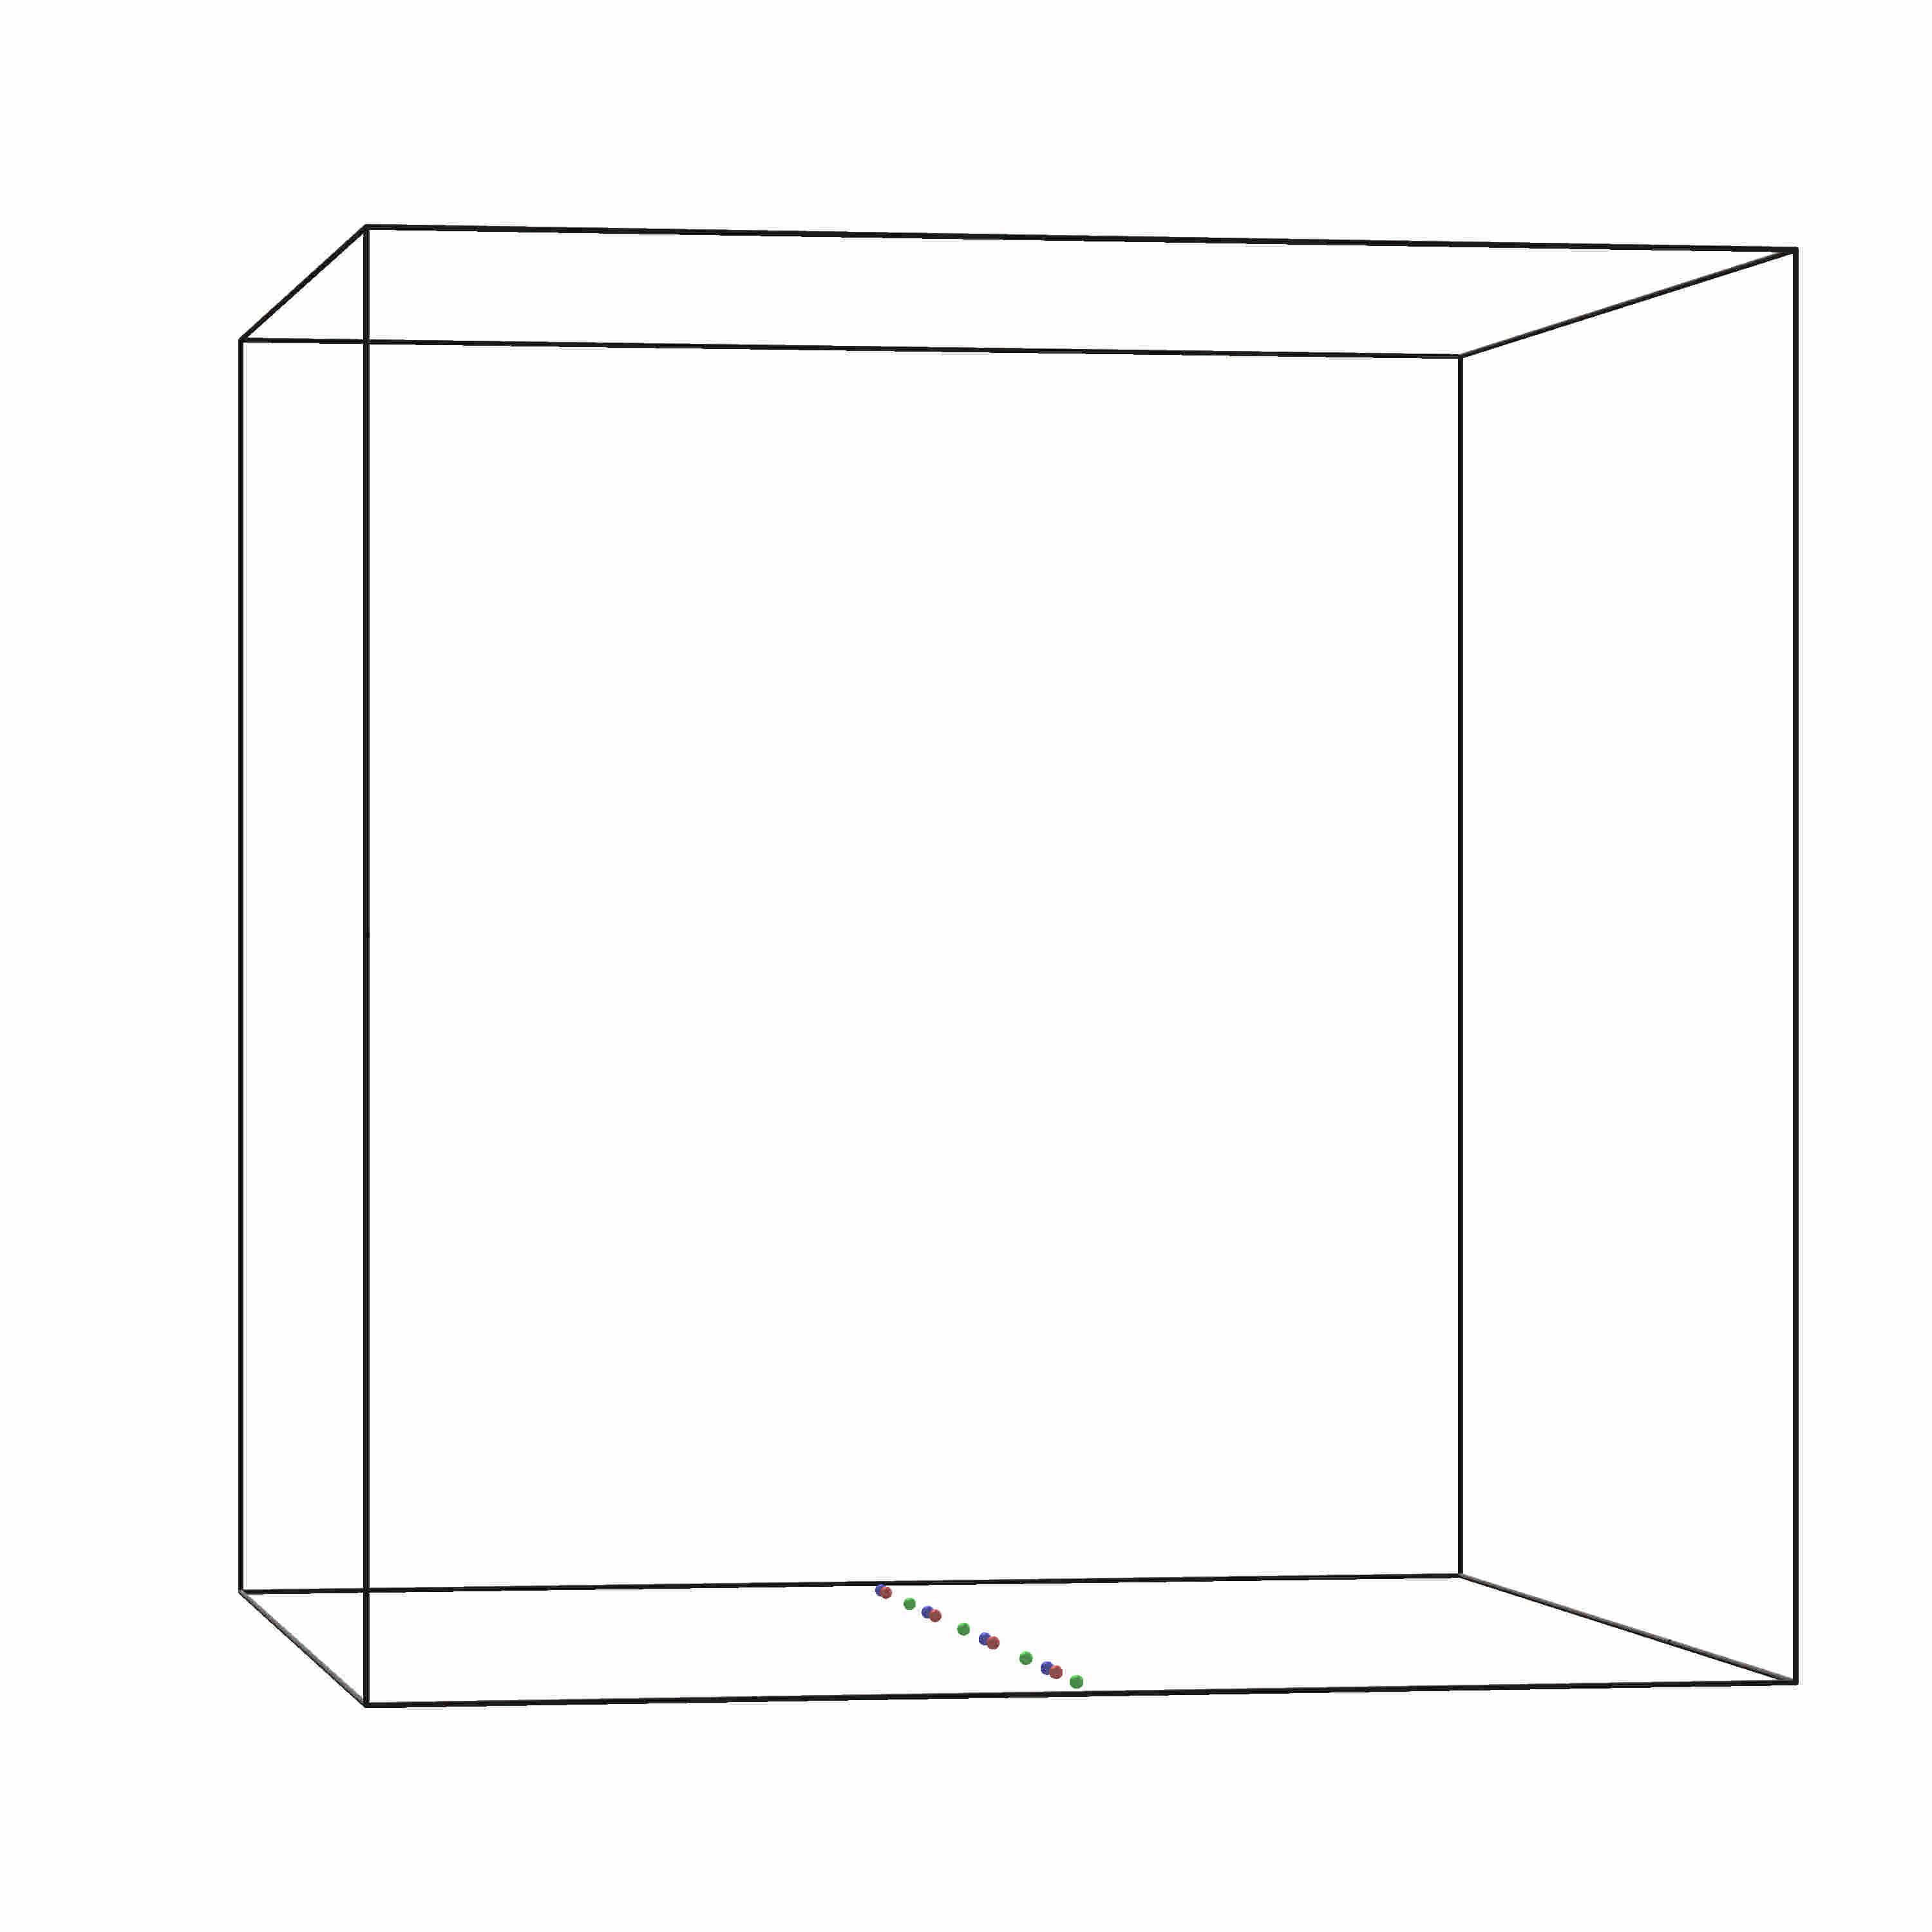
\includegraphics[width=1.1\textwidth]{image1000001}
                \label{p11a}
        \end{subfigure}\vspace*{-2em}
\centering
        \begin{subfigure}[b]{\textwidth}
               \includegraphics[width=1.1\textwidth]{1000050}
                        \label{p11b}
        \end{subfigure}\vspace*{-2em}
                \centering
        \begin{subfigure}[b]{\textwidth}
                \includegraphics[width=1.13\textwidth]{1000150}
                \label{p11c}
        \end{subfigure}\vspace*{-2.5em}
\caption{Probability distribution for the percentage decadal change between (2085-2094) and (2005-2014) for rainfed cereal, rice, maize, groundnut and oil respectively, RCP 6 and all management levels. Left-hand plots: with CO$_2$ fertilization; right-hand plots: without CO$_2$ fertilization.}\label{p1a}
\end{figure}

\section{Alternative approach}
This involve using a kriging model, where 
\begin{equation}
\eta(x) = m(x) + Z(x)
\end{equation}
where $Z(x)$ is a stationary Gaussian process with zero mean and known covariance function. The mean $m(x) = h(x)^T\boldsymbol \beta$
$h(x)$ is assumed to be constructed by stepwise technique.
%Noninformative Bayesian analysis leads to kriging predictor and variance 

%\chapter*{Appendix}

\section*{Appendix 1: Estimation of prior hyperparameters}\label{hyper}
Noting that under GP regression, the prior distribution for the data is also a Gaussian distribution, the joint likelihood of the parameters is given as
\begin{equation}\tag{A.10}\label{like}
p(y|\boldsymbol \beta, \sigma^2, \boldsymbol{\alpha})\propto \frac{det(\bf C)^{-\frac{1}{2}}}{{(2\pi\sigma^2)}^\frac{n}{2}}\exp \Big \{\frac{(y-H\boldsymbol \beta)^T \bf C^{-1}(y-H\boldsymbol \beta)}{2\sigma^2}\Big\}
\end{equation}
where $\boldsymbol{\alpha}=[\alpha_1, \ldots, \alpha_n]$ is a vector of correlation lengths and $det(\bf C)$ is the determinant of correlation matrix $\bf C$, integrating out $\boldsymbol \beta$ using a non-informative (uniform) prior such that $p(\boldsymbol \beta) \propto$ 1. We have a marginal likelihood
\begin{equation}\tag{A.10b}\label{like2}
p(\by|\sigma^2, \boldsymbol{\alpha})\propto \frac{\det(\bf C)^{-\frac{1}{2}}\det(H^TCH)^{-\frac{1}{2}}}{{(2\pi\sigma^2)}^\frac{n-p}{2}}\exp \Big \{\frac{(\by-\bH\hbbeta)^T \bC^{-1}(\by-\bH\hbbeta)}{2\sigma^2}\Big\}.
\end{equation}
Maximizing (\ref{like2}) with respect to $\boldsymbol \beta$ and $\sigma^2$ will give %the MLE of $\boldsymbol \beta$ 
\begin{equation}\tag{A.11}
\hbbeta=(\bH^T\bC^{-1}\bH)^{-1}\bH^T\bC^{-1}\by
\end{equation}

\begin{equation}\tag{A.12}
\widehat{\sigma^2}=\frac{1}{n-p}\Big[\mathbf{(y-H\hat{\boldsymbol \beta})}^T\bf C^{-1}(\bf y-H\hat{\boldsymbol \beta})\Big]
\end{equation}
Now, integrate out $\sigma^2$ such that $p(\sigma^2) \propto \frac{1}{\sigma^2}$, then we have
\begin{equation}\tag{A.10c}\label{like3}
p(\by|\boldsymbol{\alpha})\propto \det(\bC)^{-\frac{1}{2}}\det(\bH^T\bC\bH)^{-\frac{1}{2}} \Big \{(\by-\bH\hbbeta)^T \bC^{-1}(\by-\bH\hbbeta)\Big\}^{-(n-p)/2}
\end{equation}
$$=\det(\bC)^{-\frac{1}{2}}\det(\bH^T\bC\bH)^{-\frac{1}{2}} {\widehat{\sigma^2}}^{-(n-p)/2}.$$
%The smoothing parameter $\boldsymbol{\alpha}$ is estimated by maximizing the marginal likelihood (\ref{like3}) using the posterior mode%, the estimates of $\hat{\boldsymbol \beta}$ and $\widehat{\sigma^2}$ are substituted in equation (\ref{like}) and maximized over $\boldsymbol \beta$ and $\sigma^2$ to obtain


The smoothing parameter $\boldsymbol{\alpha}$ is estimated from the posterior distribution using the posterior mode by the value of $\boldsymbol{\alpha}$ for which marginal likelihood (\ref{like3}) is maximised. Here, we describe briefly the maximisation of the posterior distribution of $\boldsymbol{\alpha}$ which is reparametrized as $\btau=2log(\boldsymbol{\alpha})$ to make it unconstrained optimisation. 
Therefore, function $f(\btau)=log(p(\by|\exp(\frac{\btau}{2})))$ can be optimised using a derivative-free numerical optimisation of Nelder-Mead method which is the default in the "emulator" package that we use.
%\begin{equation}\tag{A.13}
%L(\hat{\boldsymbol \beta},\widehat{\sigma^2},\boldsymbol{\alpha})=-\frac{1}{2}\Big[n~log(\widehat{\sigma^2})(\boldsymbol{\alpha})+log(det(\bf C(\boldsymbol{\alpha})))+\textnormal n\Big],
%\end{equation}
%which is a function of $\boldsymbol{\alpha}$ that can be computed using a derivative-free numerical optimisation like Nelder-Mead method see further details in %\citep{70,q10}.
%Posterior distribution is obtained as $P(\mathbf{z}|\widehat{\boldsymbol\beta},\hat\sigma^2,\hat\alpha)\sim N[m^{\bullet}(u),\sigma^2C^{\bullet}(u,u')]$, with posterior mean and covariance functions given as equations (\ref{olu1} and \ref{olu2}) respectively.







\end{document}